% Leroviditve
Az egyik legfontosabb része a projektnek a UI, mert ezt a részét látják a felhasználók és ezzel fognak interakcióba lépni. Emiatt kiemelkedően fontos, hogy az jól meg legyen tervezve. Szerencsére ennek a feladatnak a megkönnyítésére léteznek jól bevált módszerek, amelyek nagyban felgyorsítják és megkönnyítik a munkát. Az mi választásunk a Figma tervezőprogramra esett.

\section{Figma terv}
A UI terv vizuális elkészítésére a Figma\footnote{Figma: \url{https://www.figma.com}} segédprogram a legmegfelelőbb választás rengeteg szempontból. A Figma egy olyan felülettervező program, amely lehetővé teszi több felhasználó együttműködését is, például a dizájner és a fejlesztő közös munkáját. A Figmában egyszerűen, fogd és vidd módszerrel lehet hozzáadni elemeket a munkavászonhoz, de aki pontosabban szeretne tervezni, annak az oldalsávban van lehetősége pixel pontossággal megadni az elemek tulajdonságait is. A Figmában elérhetőek előre elkészített felületi elemek is, amelyek használata sokszorosan lerövidíti a tervezéshez szükséges időt. A felületi elemekhez funkcionalitást is lehet rendelni, például ha egy gombra kattint a felhasználó, akkor egy másik oldalra navigáljon.

A Figma-ban elkészített terveket követve sokkal gyorsabban lehetett fejleszteni a felhasználói felületet. Az általunk követett felhasználói weboldal terve a \ref{fig:ui-web} ábrán, az adminfelület terve a \ref{fig:ui-admin} ábrán, míg a mobilalkalmazás terve a \ref{fig:ui-mobile} ábrán látható.

\newpage
\begin{multicols*}{2}
  \begin{figure}[H]
    \centering
    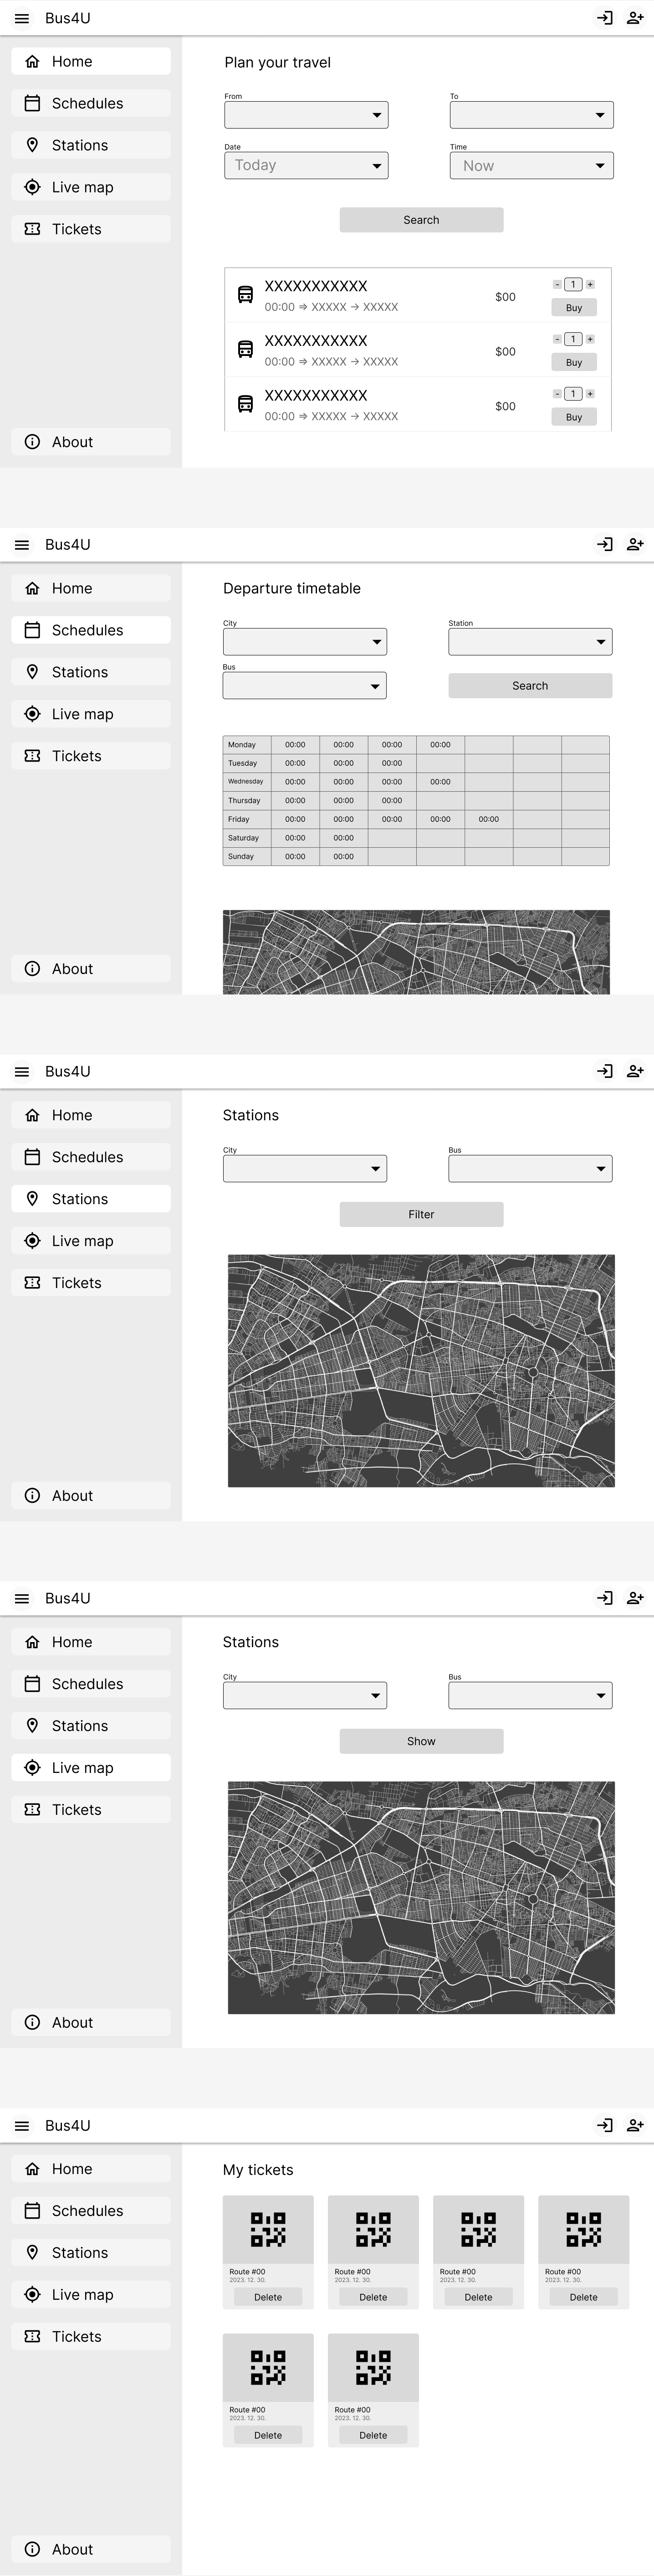
\includegraphics[height=0.9\textheight]{figures/ui-web.png}
    \caption{A felhasználói weboldal terve}
    \label{fig:ui-web}
  \end{figure}
  \begin{figure}[H]
    \centering
    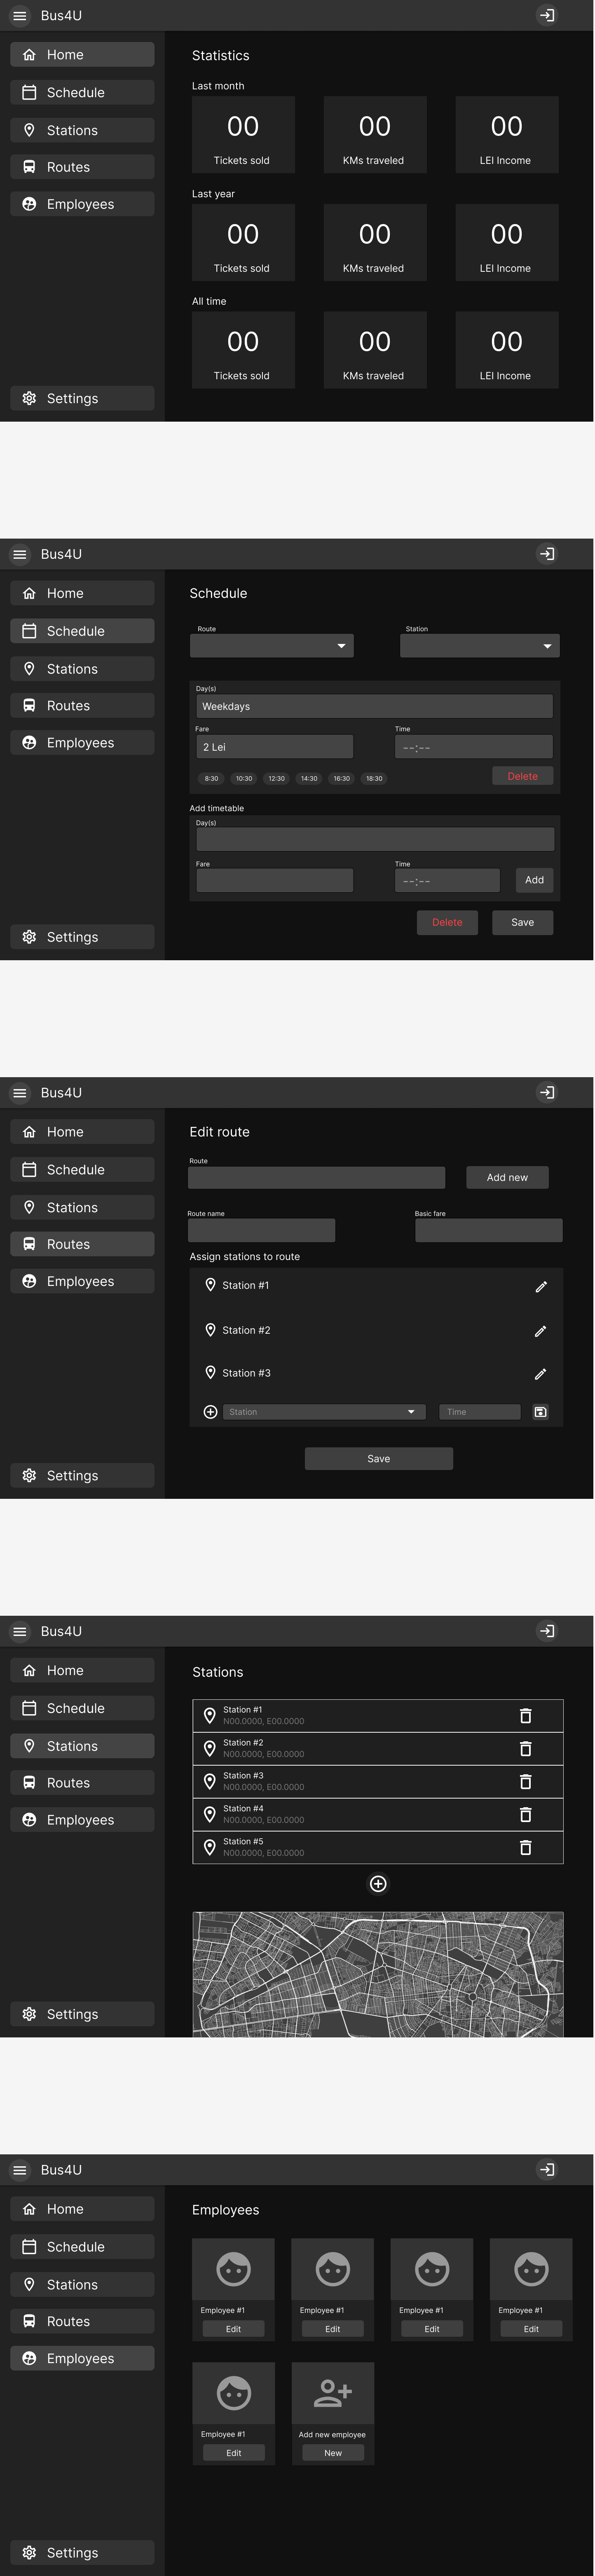
\includegraphics[height=0.9\textheight]{figures/ui-admin.png}
    \caption{Az admin weboldal terve}
    \label{fig:ui-admin}
  \end{figure}
\end{multicols*}

\begin{figure}[ht]
  \centering
  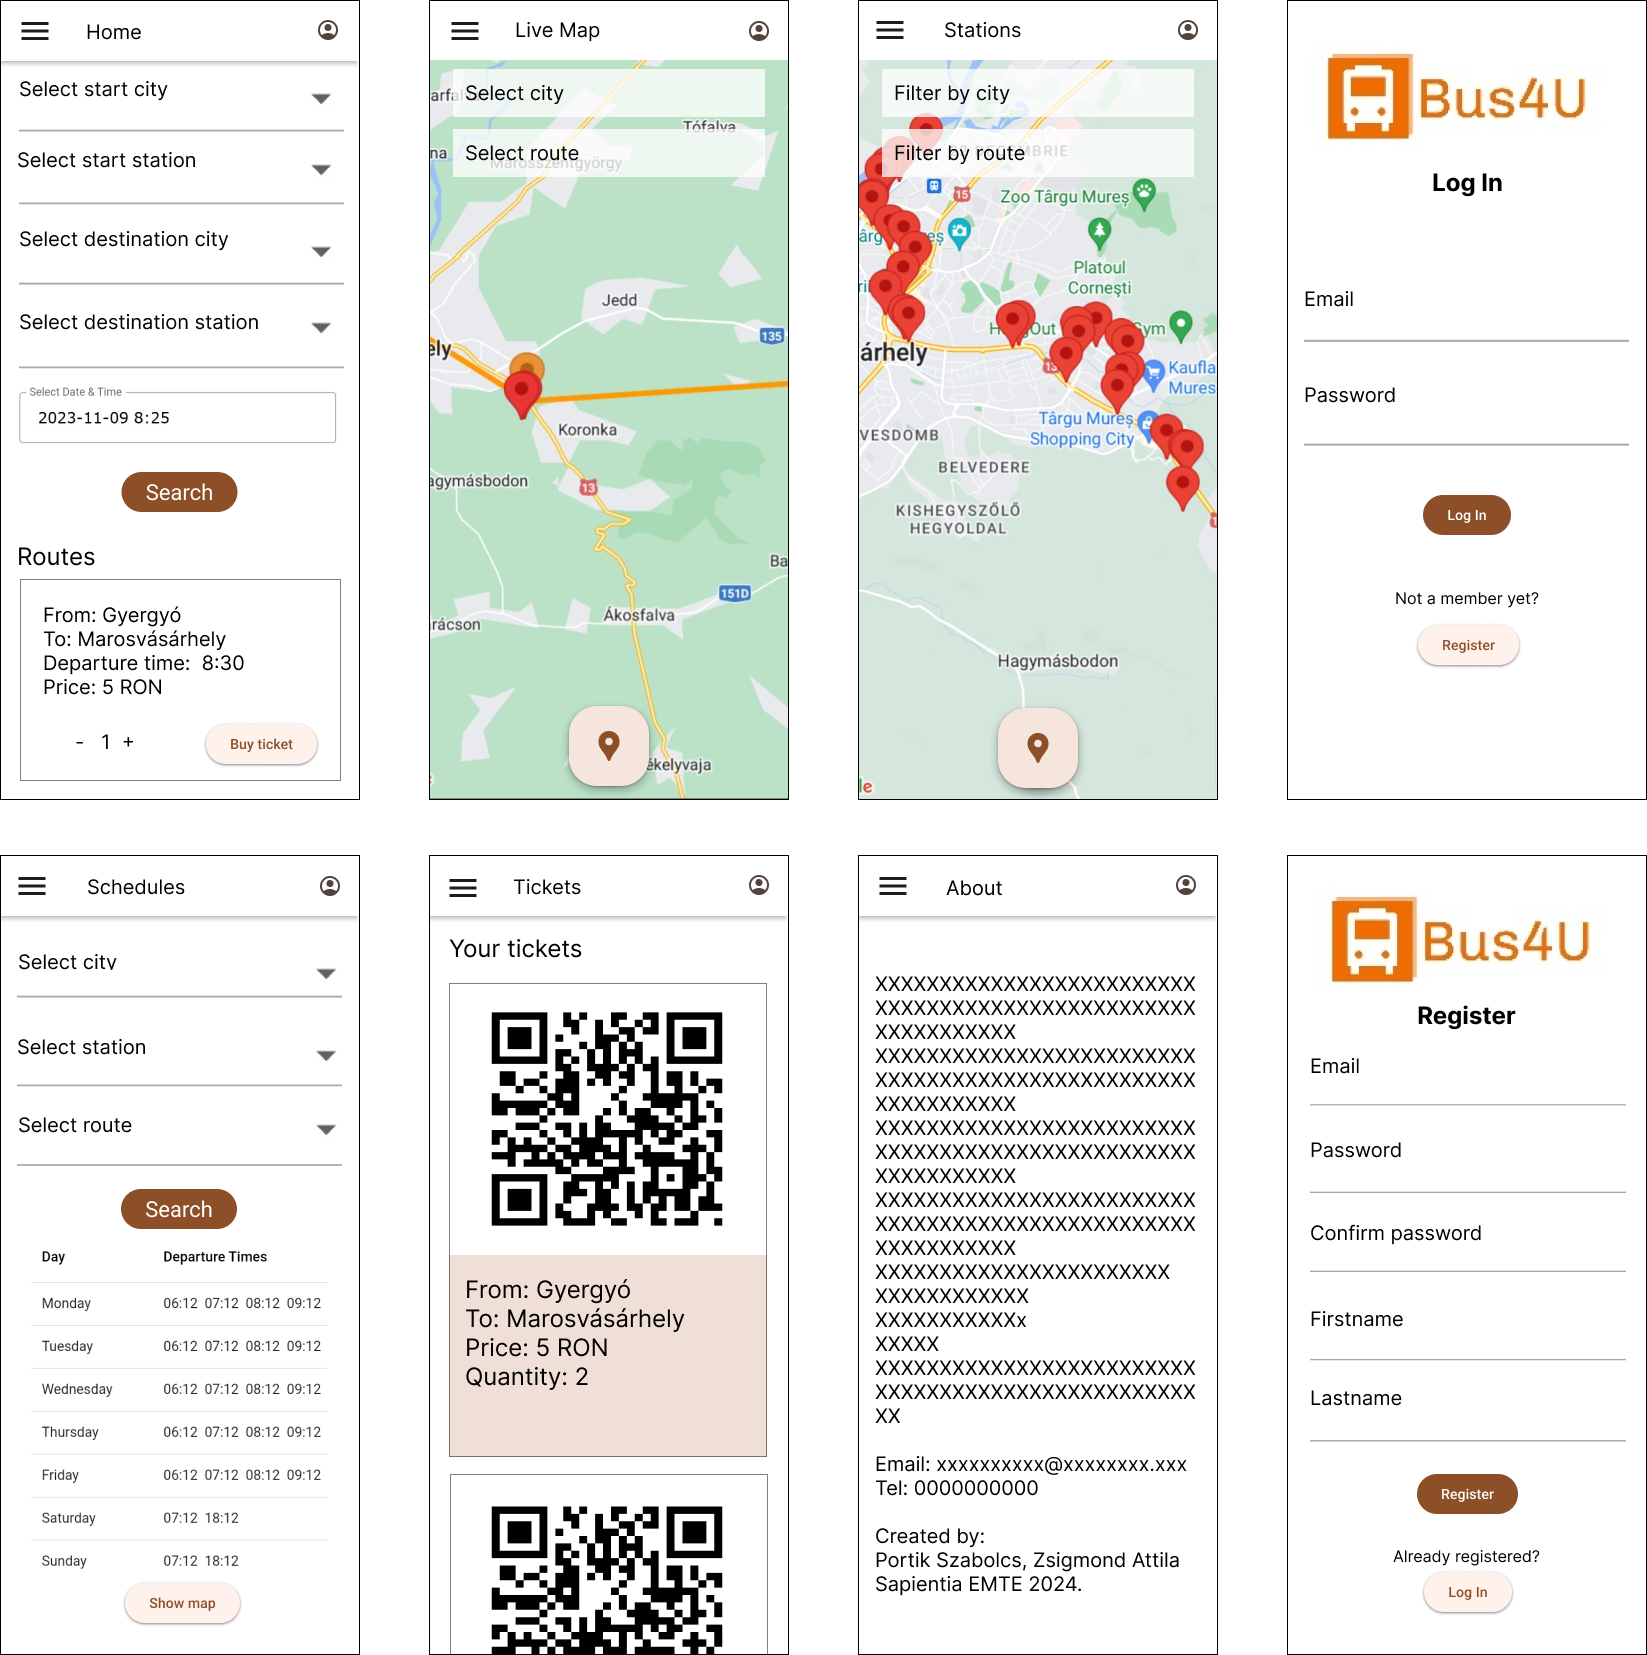
\includegraphics[width=\textwidth]{figures/ui-mobile.png}
  \caption{A mobilalkalmazás terve}
  \label{fig:ui-mobile}
\end{figure}